\chapter{V e I, Trasporto di Impedenza, Coefficiente di Riflessione, ROS}
\section{Soluzione dell'Equazione delle Linee}
\subsection{Soluzione per Onde Viaggianti}
Abbiamo quindi ricavato nel capitolo precedente le \textbf{Equazioni delle Linee}, dette anche \textbf{Soluzioni per Onde Viaggianti}:
\begin{squared}
\tag{Onde Viaggianti}
\begin{dcases}
    \frac{dV (z)}{dz} = -j \w L I (z) \\
    \frac{dI (z)}{dz} = -j \w C V (z)
\end{dcases}
\end{squared}

\subsection{Soluzione per Onde Stazionarie}
Un'altra possibile soluzione è costituita dalla combinazione lineare di due \textbf{funzioni circolari indipendenti}:
\begin{squared}[purple]
\tag{Onde Stazionarie}
\begin{dcases}
    V (z) = A\ \\cos(kz) + B \ \\sin(kz) \\
    I (z) = C\ \\cos(kz) + D \ \\sin(kz)
\end{dcases}
\end{squared}
Facilmente è possibile dimostrare che:
\begin{itemize}
    \item $A = V(0)$
    \item $C = I(0)$
    \item $B = V(\frac{\lambda}{4}) = -j Z_0 I(0)$
    \item $D = I(\frac{\lambda}{4}) = -j \frac{V(0)}{Z_0}$
\end{itemize}
(Per ricavarsi B sostituire V (z) nell'equazione delle linee e valutare in 0, analogo discorso per D).\\ \\
Poniamoci ora nella seguente situazione:
\begin{equation*}
\vcenter{\hbox{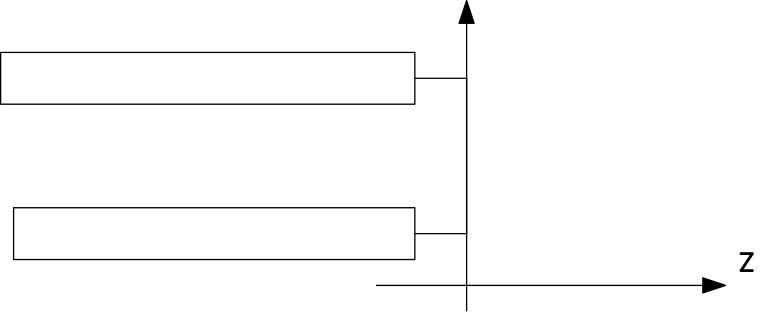
\includegraphics[width=6cm,height=4cm]{Images/figure6.png}}}
\qquad
    V(z) = -j I(0) Z_0 \\sin(kz)
\end{equation*}
E cerchiamo di disegnare il \textbf{modulo} di $|V(z)|$ cercando di capire per prima cosa dove ha gli \textbf{zeri}, ovvero quando si annulla $\\sin(kz)$:
\begin{equation*}
    kz = n \pi
\end{equation*}
Ricordando che:
\begin{equation*}
    k = \frac{2\pi}{\lambda} \ e \ che \ \lambda = \frac{2\pi}{k}
\end{equation*}
\begin{equation*}
    \implies \frac{2\pi}{\lambda} \ z = n \pi \implies z = n \ \frac{\lambda}{2}
\end{equation*}
Mentre assumerà valori massimi per:
\begin{center}
    \begin{equation*}
    z = \frac{\lambda}{4} + n \ \frac{\lambda}{2}
\end{equation*}
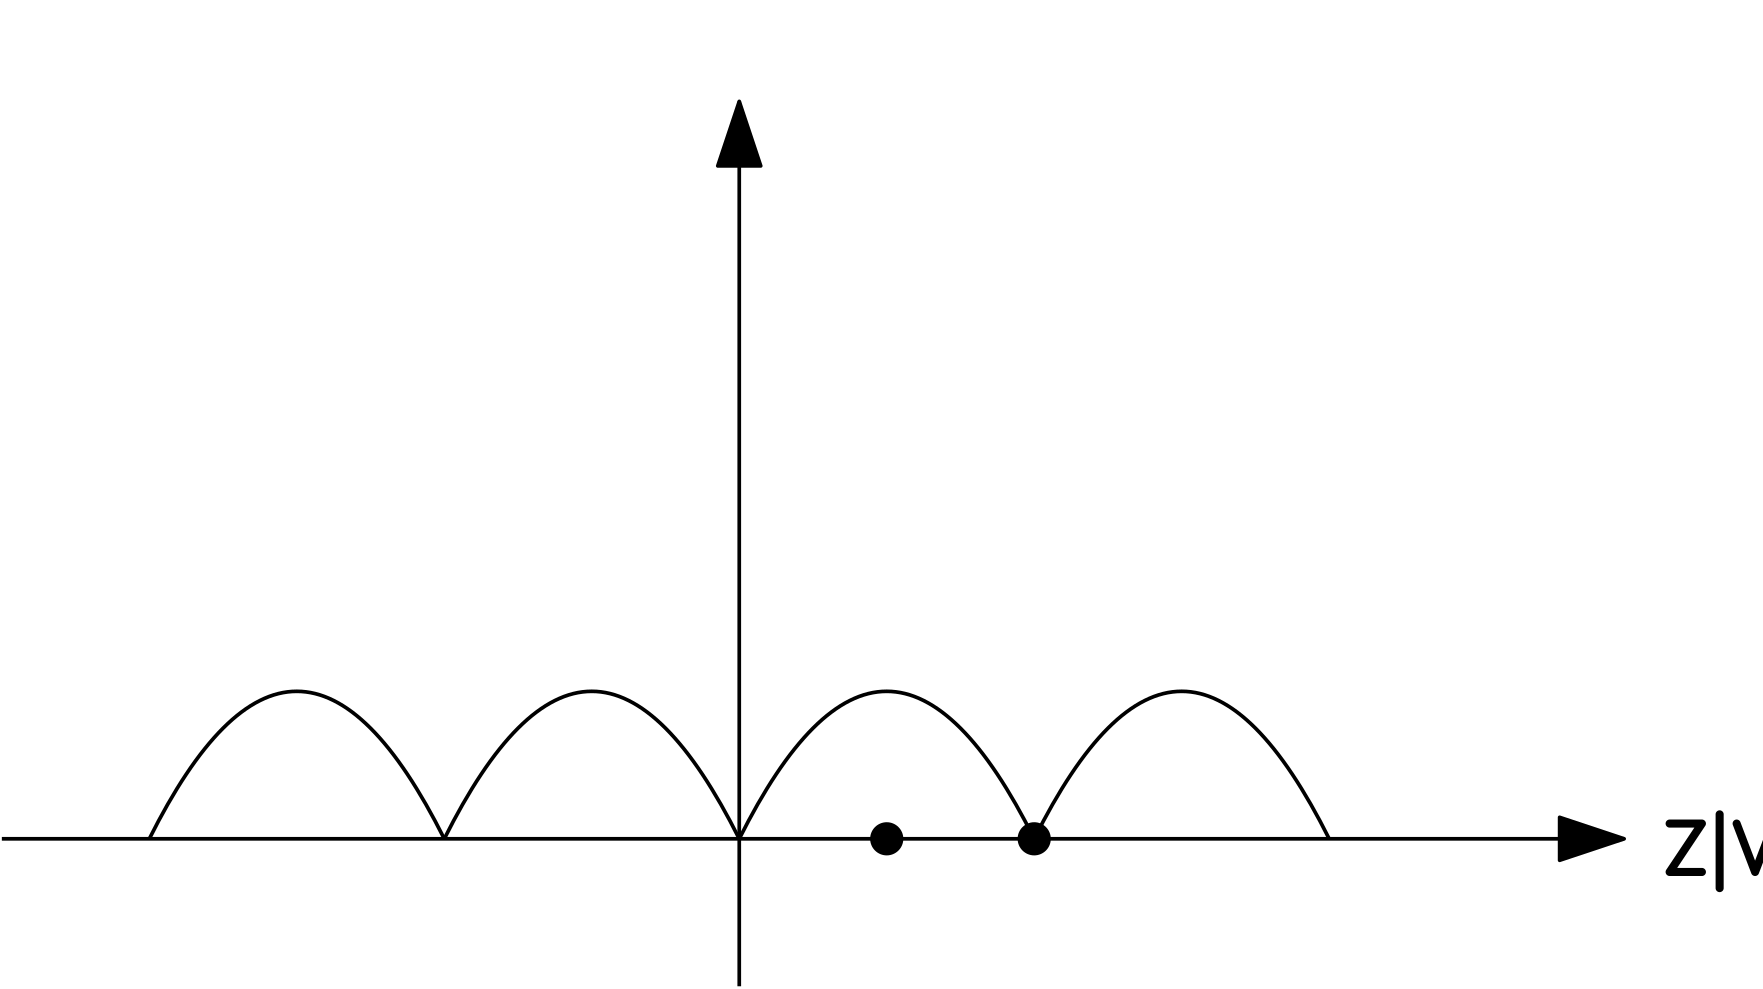
\includegraphics[width=0.6\textwidth]{Images/figure7.png}
\end{center}

Analizziamo analogamente la corrente:
\begin{equation*}
    I(z) = I(0) \\cos(kz)
\end{equation*}
Il coseno si annulla per:
\begin{equation*}
    kz = \frac{\pi}{2} + n\pi \implies \frac{2\pi}{\lambda} \ z =  \frac{\pi}{2} + n\pi \implies z = \frac{\lambda}{4} + n \ \frac{\lambda}{2}
\end{equation*}
\begin{center}
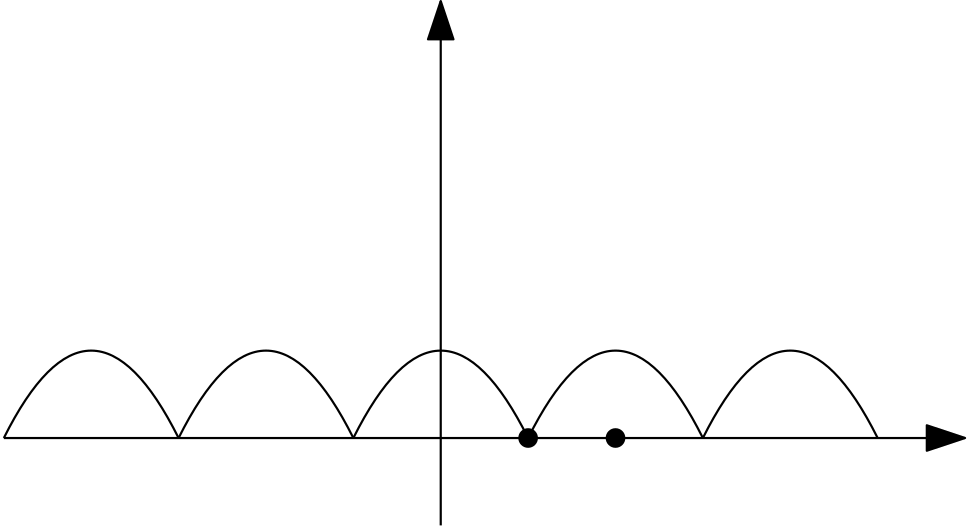
\includegraphics[width=0.6\textwidth]{Images/figure8.png}
\end{center}

\section{Trasporto dell'Impedenza}
Definiamo ora l'\textbf{impedenza} associata alla generica ascissa z dalla linea come:
\begin{squared}[green]
    Z (z) = \frac{V (z)}{I (z)} = \frac{-j \cancel{I (0)} Z_0 \sin(kz)}{\cancel{I (0)} \cos(kz)} = -j Z_0  \tan(kz)
\end{squared}
Analizziamo ora il seguente esempio di una linea chiusa su un \textbf{aperto}:
\begin{equation*}
\vcenter{\hbox{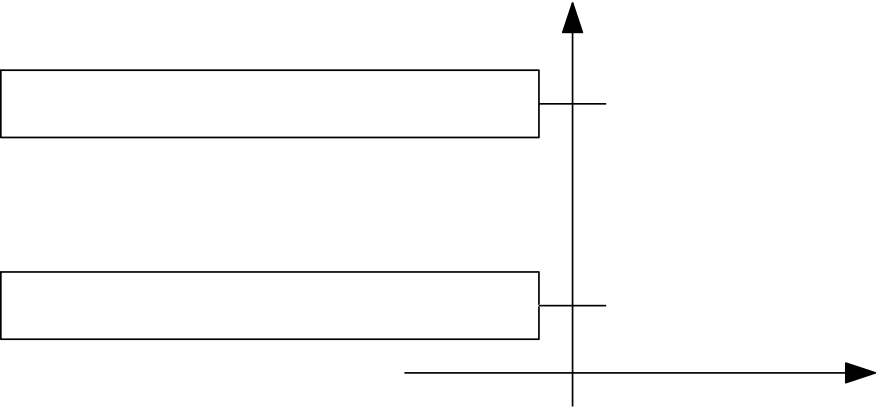
\includegraphics[width=6cm,height=4cm]{Images/figure9.png}}}
\qquad
    \begin{dcases}
        V(z) = V(0) \cos(kz)\\
        I(z) = - j \frac{V(0)}{Z_0} \sin(kz)
    \end{dcases}
\end{equation*}

In questo caso avremo i grafici invertiti:

\begin{figure}[!ht]
\centering
\begin{subfigure}{.5\textwidth}
  \centering
  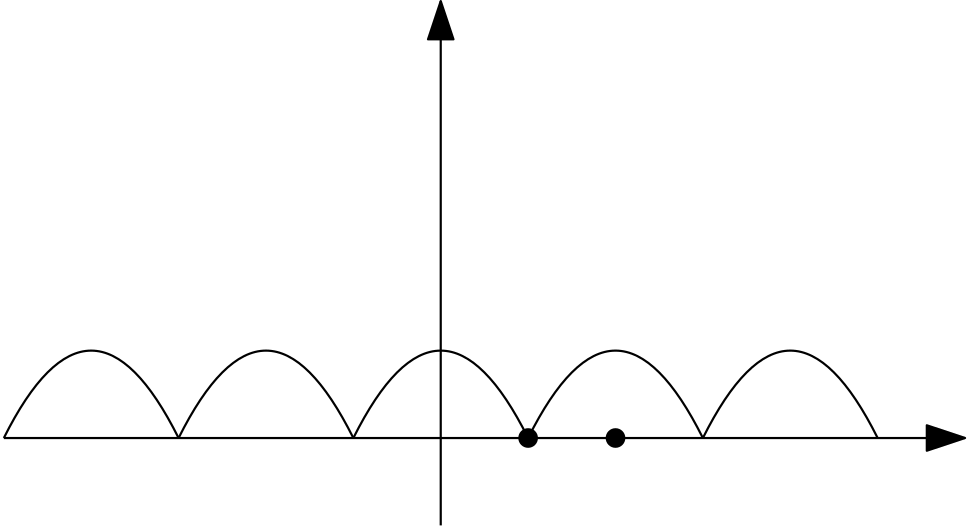
\includegraphics[width=.8\linewidth]{Images/figure8.png}
  \caption{$|V(z)|$}
\end{subfigure}%
\begin{subfigure}{.5\textwidth}
  \centering
  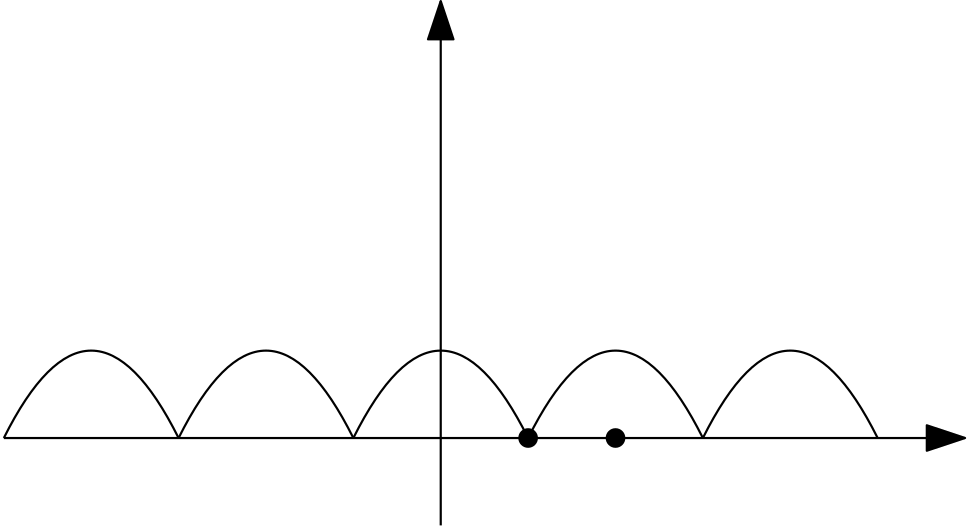
\includegraphics[width=.8\linewidth]{Images/figure8.png}
  \caption{$|I(z)|$}
\end{subfigure}
\end{figure}
\subsection{Caso Carico uguale a Impedenza della Linea}
Poniamoci nella seguente situazione:
\begin{equation*}
\vcenter{\hbox{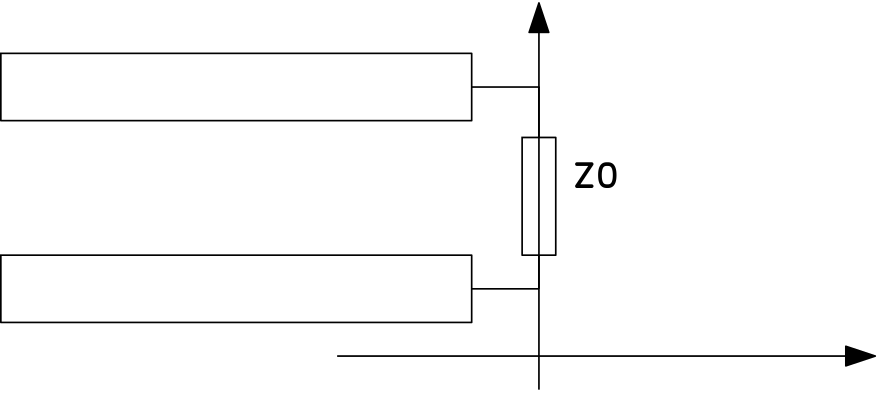
\includegraphics[width=6cm,height=3cm]{Images/figure10.png}}}
\qquad
    \begin{dcases}
        V (z) = V(0) \\cos(kz) - j Z_0 I(0) \\sin(kz)\\
        I (z) = I(0) \\cos(kz) - j \frac{V(0)}{Z_0} \\sin(kz)
    \end{dcases}
\end{equation*}
\begin{equation*}
    Z_0 = \frac{V(0)}{I(0)} \implies V(0) = Z_0 I(0)
\end{equation*}
Quindi sostituendo otteniamo:
\begin{equation*}
    \begin{dcases}
        V(z) &= Z_0 I(0) \cos(kz) - j Z_0 I(0) \sin(kz) \\
        &= Z_0 I(0) \left(\cos(kz) - j \sin(kz)\right) = Z_0 I(0) e^{-jkz}\\
        I(z) &= I(0) \cos(kz) - j  I(0) \sin(kz) = I(0) e^{-jkz}
    \end{dcases}
\end{equation*}

\subsection{Caso Impedenza Generica}
\begin{equation*}
\vcenter{\hbox{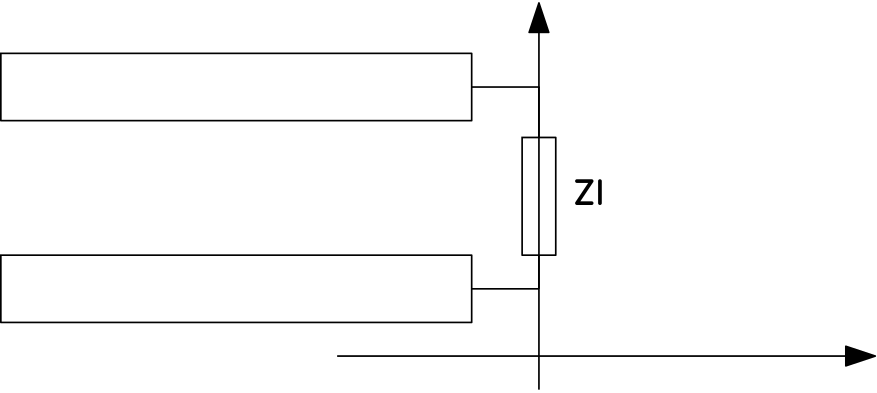
\includegraphics[width=6cm,height=3cm]{Images/figure11.png}}}
\qquad
    \begin{dcases}
        V(z) = Z_l I(0) \cos(kz) - j Z_0 I(0) \sin(kz)\\
        I(z) = I(0) \cos(kz) - j \frac{Z_l}{Z_0} I(0) \sin(kz)
    \end{dcases}
\end{equation*}
Ora calcoliamo l'\textbf{impedenza} sulla linea:
\begin{equation*}
    \begin{aligned}
    Z(z) &= \frac{ Z_l \cancel{I(0)} \cos(kz) - j Z_0 \cancel{I(0)} \sin(kz)}{\cancel{I(0)} \cos(kz) - j \frac{Z_l}{Z_0} \cancel{I(0)} \sin(kz)} = \\
    &= Z_0 \frac{Z_l \cos(kz)- j Z_0 \sin(kz)}{Z_0 \cos(kz) - j  Z_l \sin(kz) } = \\
    &\text{raccolgo sopra e sotto cos (kz)}\\
    &= Z_0 \frac{Z_l - j Z_0 \tan(kz)}{Z_0 - j Z_l \tan(kz)} = Z_0 \frac{Z_l - j Z_0 \tan(l)}{Z_0 - j Z_l \tan(l)} 
    \end{aligned}
\end{equation*}
Quindi definiamo Formula del Trasporto di Impedenza:
\begin{squared}
    Z (z) = Z_0 \frac{Z_l -j Z_0 \tan(kz)}{Z_0 -j Z_l \tan(kz)} = Z_0 \frac{Z_l -j Z_0 \tan(l)}{Z_0 -j Z_l \tan(l)} 
\end{squared}
\section{Coefficiente di Riflessione}
Consideriamo nuovamente questo caso:\\
\begin{center}
    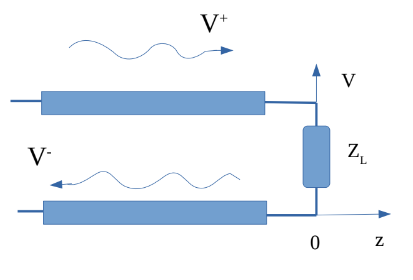
\includegraphics[width=.5\textwidth]{Images/figure12.png}\\
\end{center}
Scriviamo la tensione sottoforma di \textbf{onde viaggianti}:
\begin{equation*}
\begin{aligned}
    V(z) &= V^+ e^{-jkz} + V^- e^{jkz} = \\
    &=  V^+ e^{-jkz} \left[1 + \Gamma(z)\right]
\end{aligned}
\end{equation*}
Dove:
\begin{equation*}
    \Gamma(z) = \frac{V^-}{V^+} e^{2jkz} = \Gamma(0) e^{2jkz} 
\end{equation*}
Discorso analogo vale per la corrente:
\begin{equation*}
    I(z) = \frac{V^+}{Z_0} e^{-jkz} \left[1 - \Gamma(z)\right]
\end{equation*}
Mentre:
\begin{equation*}
\begin{aligned}
    Z(z) &= \frac{V(z)}{I(z)} = Z_0 \frac{1 + \Gamma(z)}{1- \Gamma(z)} \\
    Z(0) &= \frac{V(0)}{I(0)} = Z_0 \frac{1 + \Gamma(0)}{1- \Gamma(0)}
\end{aligned}
\end{equation*}
Possiamo inoltre definire:
\begin{equation*}
    \Gamma(0) = \frac{Z_l - Z_0}{Z_l + Z_0}
\end{equation*}

\subsection{Caratteristiche del Coefficiente di Riflessione}
Lungo una linea \textbf{senza perdite} abbiamo che:
\begin{equation*}
    \Gamma(z) = \frac{V^-}{V^+} e^{2jkz} = \Gamma(0) e^{2jkz} 
\end{equation*}
Allora se facciamo il \textbf{modulo}:
\begin{equation*}
    |\Gamma(z)| = |\Gamma(0) e^{2jkz}| = |\Gamma(0)| |e^{2jkz}| = |\Gamma(0)|
\end{equation*}
Vuol dire che il \textbf{modulo del Coefficiente di Riflessione non varia lungo una linea uniforme}.\\ \\

Ora scriviamo:
\begin{equation*}
    \Gamma_l = \frac{Z_l - Z_0}{Z_l + Z_0} = \frac{R_l + jX_l - Z_0}{R_l + jX_l + Z_0}
\end{equation*}
Facciamo il modulo quadro:
\begin{equation*}
    |\Gamma_l|^2 =  \frac{{(R_l - Z_0)}^2 + X_l^2 }{{(R_l + Z_0)}^2 + X_l^2}
    \begin{cases}
    = 0  \leftrightarrow Z_l = Z_0\\
    = 1  \leftrightarrow Z_l = jX_l\\
    < 1  \; altrimenti
    \end{cases}
\end{equation*}
\section{Rapporto d'Onda Stazionario}
Si definisce il \textbf{Rapporto d'Onda Stazionario} (ROS) lungo una linea omogenea il rapporto:

\begin{squared}[yellow]
    ROS = \frac{|V|_{\max}}{|V|_{\min}}
\end{squared}
Possiamo metterlo in relazione con il modulo del \textbf{Coefficiente di Riflessione}:
\begin{equation*}
    \begin{aligned}
    V(z) = V^+ e^{-jkz} + V^- e^{jkz} = V^+ e^{-jkz} \left(1 + \Gamma(0) e^{2jkz}\right) 
    \end{aligned}
\end{equation*}
\begin{equation*}
    \begin{aligned}
    |V(z)| &= |V^+ e^{-jkz} + V^- e^{jkz}| = |V^+ e^{-jkz}| \ |\left(1 + \Gamma(0) e^{2jkz}\right)| = \\
    &=|V^+| \ |\left(1 + \Gamma(0) e^{2jkz}\right)| 
    \end{aligned}
\end{equation*}
Quindi il ROS lo scriveremo come:
\begin{equation*}
\begin{aligned}
    ROS &= \frac{|V|_{\max}}{|V|_{\min}} = \frac{{(\cancel{|V^+|} \ |\left(1 + \Gamma(0) e^{2jkz}\right)|)}_{\max}}{{(\cancel{|V^+|} \ |\left(1 + \Gamma(0) e^{2jkz}\right)|)}_{\min}} = \\
    &= \frac{{|\left(1 + \Gamma(0) e^{2jkz}\right)|}_{\max}}{|\left(1 + \Gamma(0) e^{2jkz}\right)|_{\min}}
\end{aligned}
\end{equation*}
Possiamo riscrivere:
\begin{equation*}
    \Gamma(0) = |\Gamma(0)| e^{j \Phi_0}
\end{equation*}
Quindi:
\begin{equation*}
    \Gamma(z) = \Gamma(0) e^{2jkz} = |\Gamma(0)| e^{j \Phi_0} e^{2jkz} = |\Gamma(0)| e^{j(2jkz + \Phi_0)} 
\end{equation*}
Quindi $\Gamma(z)$ ha:
\begin{itemize}
    \item $|\Gamma(z)| = |\Gamma(0)|$
    \item $ARG(\Gamma(z)) = (2kz + \Phi_0)$
\end{itemize}
Inoltre notiamo che $\Gamma(z)$ è \textbf{periodica}:
\begin{equation*}
    2kz = 2\pi \implies 2 \ \frac{2\pi}{\lambda} z = 2\pi \implies z = \frac{\lambda}{2}
\end{equation*}
Quindi il numeratore del ROS è massimo quando:
\begin{equation*}
    2kz + \Phi_0 = 2n\pi
\end{equation*}
Possiamo allora definire una serie di ascisse $z_n$ in corrispondenza delle quali la \textbf{tensione è massima}:
\begin{equation*}
    z_n = \frac{n\pi}{k} - \frac{\Phi_0}{2k} = n \ \frac{\lambda}{2} - \frac{\Phi_0}{2\pi} \frac{\lambda}{2} = \left(n - \frac{\Phi_0}{2\pi}\right) \frac{\lambda}{2} 
\end{equation*}
\begin{equation*}
\begin{aligned}
    |V|_{\max} &= |V^+| \ |1 + |\Gamma(0) e^{j(2kz_n + \Phi_0)}| =\\
    &= |V^+| \ (1 + |\Gamma(0)|) =|V^+| \ (1 + |\Gamma(z)|)
\end{aligned}
\end{equation*}
Un discorso analogo può essere fatto per minimizzare il denominatore del ROS\@:
\begin{equation*}
    2kz + \Phi_0 = \pi + 2n\pi = (2n+1)\pi
\end{equation*}
\begin{equation*}
    z_n' = \frac{n\pi}{k} + \frac{\pi}{2k} - \frac{\Phi_0}{2k} = n \ \frac{\lambda}{2} + \frac{\lambda}{4} - \frac{\Phi_0}{2\pi}  \frac{\lambda}{2} = \left(n + \frac{1}{2} - \frac{\Phi_0}{2\pi}\right) \frac{\lambda}{2} 
\end{equation*}
\begin{equation*}
\begin{aligned}
    |V|_{\min} &= |V^+| \ |1 + |\Gamma(0) e^{j(2k z_n' + \Phi_0)}| =\\
    &= |V^+| \ (1 - |\Gamma(0)|) =|V^+| \ (1 - |\Gamma(z)|)
\end{aligned}
\end{equation*}
Quindi in conclusione:
\begin{squared}[violet]
    ROS = \frac{1 + |\Gamma(z)|}{1 -|\Gamma(z)|}
\end{squared}
Quindi al variare del carico $Z_l$ il ROS varia per:
\begin{equation*}
    1 \leq ROS \leq \infty
\end{equation*}
In particolare:
\begin{itemize}
    \item $ROS = 1$ se $\Gamma = 0$ ovvero se $Z_l = Z_0$
    \item $ROS = \infty$ se $|\Gamma|=1$ ovvero se $Z_l = j X_l$
\end{itemize}
Calcoliamo ora l'impedenza in $z_n$:
\begin{equation*}
    Z(z_n) = \frac{V(z_n)}{I(z_n)} = Z_0 \frac{\cancel{V^+} (1 + |\Gamma|)}{\cancel{V^+} (1 - |\Gamma|)} = Z_0 \ ROS
\end{equation*}
Facciamo un analogo calcolo per $z_n'$:
\begin{equation*}
    Z(z_n') = \frac{V(z_n')}{I(z_n')} = Z_0 \frac{\cancel{V^+} (1 - |\Gamma|)}{\cancel{V^+} (1 + |\Gamma|)} = \frac{Z_0}{ROS}
\end{equation*}
Quindi $|Z|$ assume valori:
\begin{equation*}
    \frac{Z_0}{ROS} \leq |Z(z)| \leq Z_0 \ ROS
\end{equation*}
Ora definiamo la parte reale dell'impedenza lungo la linea come:
\begin{equation*}
    R(z) = Re\{Z(z)\} = Z_0 Re\left\{\frac{1 + \Gamma(z)}{ 1 - \Gamma(z)}\right\}
\end{equation*}
\begin{equation*}
\begin{aligned}
    Re\left\{\frac{1 + \Gamma(z)}{ 1 - \Gamma(z)}\right\} &=  Re\left\{\frac{(1 + \Gamma(z)) \ (1 - \Gamma^*(z)) }{ {|1 - \Gamma(z)|}^2}\right\} = \\
    &= Re\left\{\frac{1 - {|\Gamma(z)|}^2 + 2j Im\{\Gamma(z)\}}{ {|1 - \Gamma(z)|}^2}\right\} = \frac{1 - {|\Gamma(z)|}^2}{{|1 - \Gamma(z)|}^2} 
\end{aligned}
\end{equation*}
Quindi:
\begin{equation*}
    R(z) = Z_0 \frac{1 - {|\Gamma(z)|}^2}{{|1 - \Gamma(z)|}^2} 
\end{equation*}
Dove $|\Gamma(z)|^2$ è costante per qualsiasi z, quindi varierà solo il suo denominatore:
\begin{equation*}
    Z_0 \frac{1 - |\Gamma(z)|^2}{{[1 + |\Gamma(z)|]}^2}  \leq R(z) \leq Z_0 \frac{1 + |\Gamma(z)|^2}{{[1 - |\Gamma(z)|]}^2} 
\end{equation*}
Ovvero
\begin{equation*}
    \frac{Z_0}{ROS}  \leq R(z) \leq Z_0 ROS
\end{equation*}







